\documentclass[11pt,a4paper]{article}
\usepackage{shared-style}
\usepackage{listings}
\usepackage{graphicx}
\usepackage{amsmath}
\usepackage{hyperref}

\shorttitle{Reinforcement Learning}
\shortauthors{Maltoni and de Mingo Arroyo}

\begin{document}

\papertitle{Reinforcement Learning: Training an Agent in the Gymnasium}
\paperauthors{Adam Maltoni and Ib\'on de Mingo Arroyo}
\paperdate{May 2025}

\begin{abstract}
This lab assignment explores reinforcement learning by training an agent in the Gymnasium environment. We implement and compare Q-learning and SARSA algorithms across various environments, analyze the effects of exploration parameters, and introduce Deep Q-Learning (DQN) for more complex state spaces.
\end{abstract}

\tableofcontents
\newpage

\section{Exercise 1: The gymnasium}

Training a reinforcement learning agent at the gymnasium. 
\begin{itemize}
    \item Basic usage: \url{https://gymnasium.farama.org/introduction/basic_usage/}
    \item Training an RL-agent: \url{https://gymnasium.farama.org/introduction/train_agent/}
\end{itemize}

\begin{lstlisting}[language=Python]
%load_ext autoreload
%autoreload 2
import numpy as np
import matplotlib.pyplot as plt
import gymnasium as gym
import imageio
import os
from tqdm.notebook import tqdm
import rl_utils
import time
from IPython.display import display, clear_output
from reinforcement_learning import (
    sarsa_learning,
    q_learning, 
    greedy_policy,
    epsilon_greedy_policy,
)
\end{lstlisting}

\begin{lstlisting}[language=Python]
import gymnasium as gym
env = gym.make('CartPole-v1')
\end{lstlisting}

\begin{lstlisting}[language=Python]
env = gym.make("LunarLander-v3", render_mode="human")
observation, info = env.reset()
episode_over = False
while not episode_over:
    action = env.action_space.sample()  # agent policy that uses the observation and info
    observation, reward, terminated, truncated, info = env.step(action)
    episode_over = terminated or truncated
env.close()
\end{lstlisting}

\section{Exercise 2: Q-learning}

We're now ready to code our Q-Learning algorithm.

\subsection{Step 0: Set up and understand Frozen Lake environment}
Let's begin with a simple 4x4 map and non-slippery, meaning the agent always moves in the desired direction.
We add a parameter called \texttt{render\_mode} that specifies how the environment should be visualised. In our case because we want to record a video of the environment at the end, we need to set \texttt{render\_mode} to \texttt{rgb\_array}.

As explained in the documentation \texttt{rgb\_array}: Return a single frame representing the current state of the environment. A frame is a \texttt{np.ndarray} with shape (H, W, 3) representing RGB values for an H (height) times W (width) pixel image.

\begin{lstlisting}[language=Python]
small_environment = gym.make(
    'FrozenLake-v1', 
    map_name='4x4', 
    is_slippery=False, 
    render_mode='rgb_array',
)
\end{lstlisting}

Let's see what the environment looks like:

\begin{lstlisting}[language=Python]
state, info = small_environment.reset()  # observation state
action_names = {0: 'Left', 1: 'Down', 2: 'Right', 3: 'Up'}
print(state)
print(info, '(Probability that the action has led to the current state)')
n_states = small_environment.observation_space.n
print("There are ", n_states, " possible states")
\end{lstlisting}

\begin{lstlisting}[language=Python]
n_actions = small_environment.action_space.n
print("There are ", n_actions, " possible actions")
print(action_names)
fig, ax = plt.subplots()
game_image = ax.imshow(small_environment.render())
\end{lstlisting}

\begin{lstlisting}[language=Python]
# Generate a random observed state
print("Observation state (randomly selected)", 
small_environment.observation_space.sample()) 
# Generate a random action from the current state
print("Action (randomly selected):", 
small_environment.action_space.sample())
\end{lstlisting}

\begin{lstlisting}[language=Python]
# Generate an episode
obsevation, info = small_environment.reset()  # state state_state
fig, ax = plt.subplots()
game_image = ax.imshow(small_environment.render())
MAX_STEPS = 100
refresh_rate = 1 # in (1 / seconds)
episode_over = False
n_steps = 0
   
while not episode_over and n_steps < MAX_STEPS:
    n_steps += 1
    action = small_environment.action_space.sample()  
    state, reward, terminated, truncated, info = small_environment.step(action)
    episode_over = terminated or truncated
    
    ax.set_title(
        'Step: {}  State: {}  Reward: {} Action:{}'.format(
            n_steps, 
            state,
            reward,
            action_names[action],
        )
    )
    
    display(fig)
    time.sleep(1.0 / refresh_rate)
    clear_output(wait=True)  # Clear previous output
    game_image.set_data(small_environment.render())
    
small_environment.close()
\end{lstlisting}

\subsection{Step 1: Greedy and Epsilon greedy policies}

Since Q-Learning is an off-policy algorithm, we have two policies. This means we're using a different policy for acting and updating the value function.

\begin{itemize}
    \item Epsilon-greedy policy (acting policy)
    \item Greedy-policy (updating policy)
\end{itemize}

The greedy policy will also be the final policy we'll have when the Q-learning agent completes training. The greedy policy is used to select an action using the Q-table.

Epsilon-greedy is the training policy that handles the exploration/exploitation trade-off.
\begin{itemize}
    \item With probability $1 - \epsilon$: we do exploitation (i.e. our agent selects the action with the highest state-action pair value).
    \item With probability $\epsilon$: we do exploration (trying a random action).
\end{itemize}

As the training continues, we progressively reduce the epsilon value since we will need less and less exploration and more exploitation.

\subsection{Step 2: Train the RL agent}

\textbf{TO DO}: Implement the Q-learning algorithm in \texttt{reinforcement\_learning.py}

Define the hyperparameters for the learning process. The exploration related hyperparameters are some of the most important ones.

\begin{itemize}
    \item We need to make sure that our agent explores enough of the state space to learn a good value approximation. To do that, we need to have progressive decay of the epsilon.
    \item If you decrease epsilon too fast (too high decay\_rate), you take the risk that your agent will be stuck in a local optimum, since your agent didn't explore enough of the state space and hence can't solve the problem.
\end{itemize}

\begin{lstlisting}[language=Python]
# Training hyperparameters
n_training_episodes = 1000
max_steps = 100 # Maximum number of steps per episode
learning_rate = 0.7          
gamma = 0.95 # Discount factor
# Exploration parameters
max_epsilon = 1.0  # Initial exploration probability
min_epsilon = 0.05  # Minimum exploration probability
decay_rate = 0.0005 # Exponential decay rate for the exploration probability

# Initialize Q-table
Qtable_small = np.zeros(
    (
        small_environment.observation_space.n, 
        small_environment.action_space.n
    )
)
# Learn Q-table
Qtable_small = q_learning(
    small_environment, 
    n_training_episodes,
    max_steps,
    learning_rate,
    gamma,
    min_epsilon, 
    max_epsilon, 
    decay_rate,  
    Qtable_small,
)
\end{lstlisting}

\begin{lstlisting}[language=Python]
frames = rl_utils.generate_greedy_episode(small_environment, Qtable_small)
rl_utils.show_episode(frames, interval=250)
\end{lstlisting}

\subsection{A more challenging problem}
We're ready now to find our way in more challenging environments.

\begin{lstlisting}[language=Python]
large_environment = gym.make(
    'FrozenLake-v1', 
    map_name='8x8', 
    is_slippery=False, 
    render_mode='rgb_array'
)
n_states = large_environment.observation_space.n
print("There are ", n_states, " possible states")
n_actions = large_environment.action_space.n
print("There are ", n_actions, " possible actions")
\end{lstlisting}

\begin{lstlisting}[language=Python]
n_training_episodes = 30000
max_steps = 500
learning_rate = 0.5
gamma = 0.99
max_epsilon = 1.0
min_epsilon = 0.2
decay_rate = 0.0001
# Initialize Q-table
Qtable_large = np.zeros(
    (
        large_environment.observation_space.n, 
        large_environment.action_space.n
    )
)
# Learn Q-table
Qtable_large = q_learning(
    large_environment, 
    n_training_episodes,
    max_steps,
    learning_rate,
    gamma,
    min_epsilon, 
    max_epsilon, 
    decay_rate,  
    Qtable_large,
)
\end{lstlisting}

\begin{lstlisting}[language=Python]
frames = rl_utils.generate_greedy_episode(large_environment, Qtable_large)
rl_utils.show_episode(frames, interval=250)
\end{lstlisting}

\subsection{Slippery environment}
Our environment is now slippery, meaning the agent sometimes slips and moves in an unintended direction.

\begin{lstlisting}[language=Python]
slippery_environment = gym.make(
    'FrozenLake-v1', 
    map_name='8x8', 
    is_slippery=True, 
    render_mode='rgb_array',
)
\end{lstlisting}

To visualize the challenges in this environment, let's make our agent go right several times and see what happens:

\begin{lstlisting}[language=Python]
go_right = []
action = 2  # go-right
n_steps = 20
state, info = slippery_environment.reset()
for i in range(n_steps):
    go_right.append(slippery_environment.render())  # Capture current frame
    slippery_environment.step(action)
rl_utils.show_episode(go_right, interval=250)
\end{lstlisting}

Let's see what happens when we train our agent in the same way as before.

\begin{lstlisting}[language=Python]
# TO DO: Training hyperparameters
n_training_episodes = 30000
max_steps = 700 
learning_rate =  0.7         
gamma =  0.99 
max_epsilon =  1 
min_epsilon =  0.1 
decay_rate =  0.00001

Qtable_slippery = np.zeros((slippery_environment.observation_space.n, slippery_environment.action_space.n))
Qtable_slippery = q_learning(
    slippery_environment, 
    n_training_episodes,
    max_steps,
    learning_rate,
    gamma,
    min_epsilon, 
    max_epsilon, 
    decay_rate,
    Qtable_slippery,
)
\end{lstlisting}

Now we fix it:

\begin{lstlisting}[language=Python]
# TO DO: Training hyperparameters
n_training_episodes = 100000
max_steps = 800 
learning_rate =  0.1         
gamma =  0.995 
max_epsilon =  1 
min_epsilon =  0.5 
decay_rate =  0.00001

Qtable_slippery = np.zeros((slippery_environment.observation_space.n, slippery_environment.action_space.n))
Qtable_slippery = q_learning(
    slippery_environment, 
    n_training_episodes,
    max_steps,
    learning_rate,
    gamma,
    min_epsilon, 
    max_epsilon, 
    decay_rate,
    Qtable_slippery,
)
\end{lstlisting}

\section{Exercise 3: Train the RL agent using SARSA}

\textbf{TO DO}: Implement the SARSA learning algorithm in \texttt{reinforcement\_learning.py}

\begin{lstlisting}[language=Python]
slippery_environment = gym.make(
    'FrozenLake-v1', 
    map_name='8x8', 
    is_slippery=True, 
    render_mode='rgb_array',
)
n_training_episodes = 100000
max_steps = 800
learning_rate = 0.1
gamma = 0.995
max_epsilon = 1.0
min_epsilon = 0.5
decay_rate = 0.0001
# Initialize Q-table
Qtable_slippery = np.zeros(
    (
        slippery_environment.observation_space.n, 
        slippery_environment.action_space.n
    )
)
# Learn Q-table
Qtable_slippery = sarsa_learning(
    slippery_environment, 
    n_training_episodes,
    learning_rate,
    gamma,
    min_epsilon, 
    max_epsilon, 
    decay_rate,
    max_steps,
    Qtable_slippery,
)
\end{lstlisting}

\section{Exercise 4: Compare SARSA and Q-learning}

\textbf{Answer these questions:}
\begin{itemize}
    \item What is "episode reward" in RL and how is it related to the performance of an RL agent?
    \item What is "episode length" in RL and how is it related to the performance of an RL agent?
    \item What is "training error" in RL and how is it related to the performance of an RL agent?
    \item Provide an explicit expression of the training error in the cases explored.
\end{itemize}

\subsection{What is episode reward in RL and how is it related to the performance of an RL agent?}

Answer: In Reinforcement Learning (RL), the episode reward is the total cumulative reward that an agent receives during a single episode — from the initial state to a terminal state.
\begin{equation}
R^{(i)} = \sum_{t=0}^{T_i} r_t
\end{equation}
Where:
\begin{itemize}
    \item $T_i$ is the total number of time steps in episode $i$
    \item $r_t$ is the reward received at time step $t$
\end{itemize}
A higher episode reward generally indicates better performance. For example, in environments like FrozenLake, an agent receives a reward of 1 for reaching the goal. So, an episode reward of 1 means success, while 0 means failure. Tracking the average episode reward over time helps us understand how well the agent is learning.

\subsection{What is episode length in RL and how is it related to the performance of an RL agent?}

Answer: The episode length is the number of steps taken before the episode ends.
\begin{equation}
\text{Episode Length} = T
\end{equation}
Where $T$ is the total number of steps in an episode.
Episode length must be interpreted alongside the episode reward:
\begin{itemize}
    \item Short + reward = 1 $\rightarrow$ efficient path to goal
    \item Long + reward = 1 $\rightarrow$ success but with a suboptimal path
    \item Short + reward = 0 $\rightarrow$ early failure (e.g., fell into a hole)
    \item Long + reward = 0 $\rightarrow$ wandering without reaching the goal
\end{itemize}
In general, shorter episodes with higher rewards indicate that the agent is learning an effective policy.

\subsection{What is training error in RL and how is it related to the performance of an RL agent?}

Answer: The training error in RL typically refers to the Temporal Difference (TD) error, which quantifies how much the Q-value estimate changes during learning.

In Q-learning, the TD error is:
\begin{equation}
\delta_t = r_t + \gamma \cdot \max_{a'} Q(s_{t+1}, a') - Q(s_t, a_t)
\end{equation}

In SARSA, the TD error is:
\begin{equation}
\delta_t = r_t + \gamma \cdot Q(s_{t+1}, a_{t+1}) - Q(s_t, a_t)
\end{equation}

Where:
\begin{itemize}
    \item $r_t$ is the reward at time step $t$
    \item $\gamma$ is the discount factor
    \item $Q(s,a)$ is the Q-value of state $s$ and action $a$
\end{itemize}

The average training error per episode can be calculated as:
\begin{equation}
\text{Training Error} = \frac{1}{T} \sum_{t=0}^{T} |\delta_t|
\end{equation}

\begin{itemize}
    \item A high training error indicates that the agent is still learning (i.e., Q-values are changing significantly).
    \item A low training error suggests that the agent's policy is stabilizing, which often correlates with improved and consistent performance.
\end{itemize}

\section{Exercise 5: Compare SARSA and Q-learning plots}

\begin{itemize}
    \item Use matplotlib to compare the learning curves of SARSA and Q-learning, in terms of episode reward, episode length, and training error.
    \item Discuss the results obtained.
\end{itemize}

\begin{lstlisting}[language=Python]
from rl_comparatives import *
from ex5 import plot1
plot1()
\end{lstlisting}

\begin{figure}[h]
    \centering
    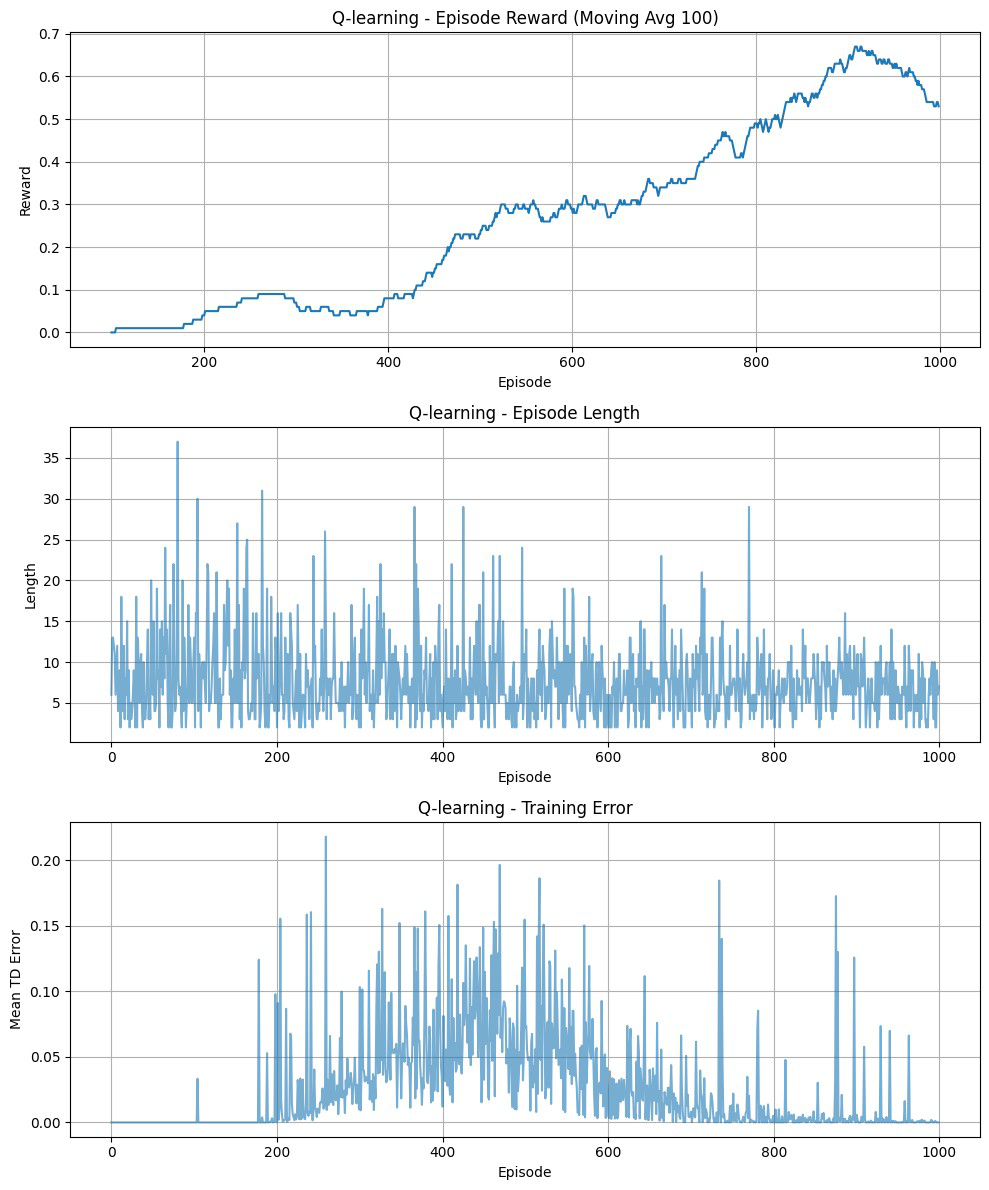
\includegraphics[width=0.8\textwidth]{img/page16_img1.png}
    \caption{Plot 1 Results}
\end{figure}

Q-learning learns faster: its average reward climbs by episode 200 and, despite a dip around 600, settles near 0.50 by episode 1000.
SARSA takes longer to improve but rises more smoothly, eventually peaking just above 0.55. Both methods cut their episode lengths from dozens of random steps down to about 4–10 moves, though Q-learning stops producing very long runs a bit sooner.

In terms of TD error, Q-learning's estimates converge to near zero around episode 700, while SARSA's error stays around 0.1–0.2 as it keeps updating on-policy. In short, Q-learning is quicker but a bit wobbly; SARSA is steadier and edges out slightly higher final rewards.

\begin{lstlisting}[language=Python]
from ex5 import plot2
plot2()
\end{lstlisting}

\begin{figure}[h]
    \centering
    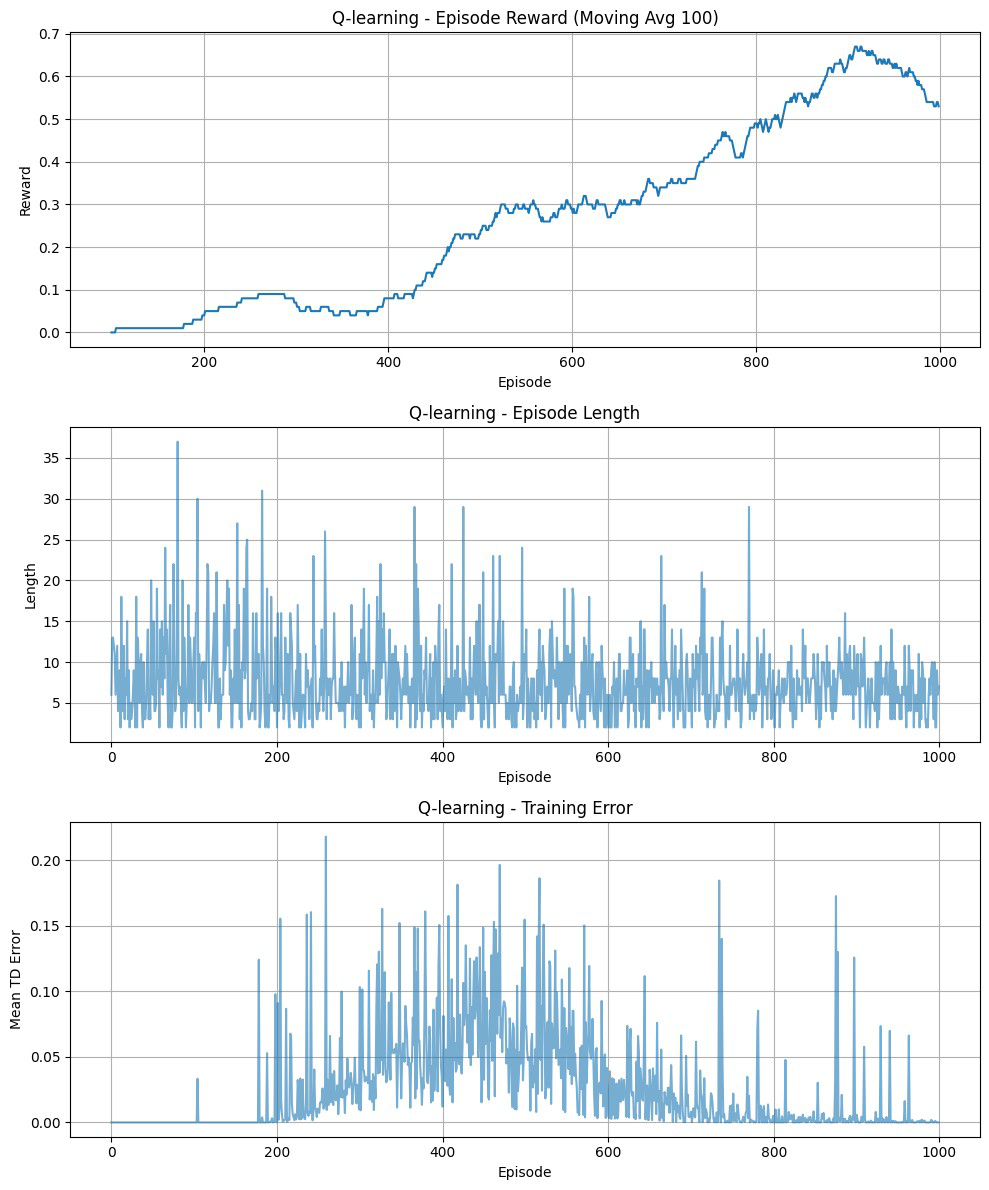
\includegraphics[width=0.8\textwidth]{img/page19_img1.png}
    \caption{Plot 2 Results}
\end{figure}

In the FrozenLake environment, Q-learning learned successfully: rewards increased, episode lengths dropped, and training error decreased over time. SARSA, however, failed to learn—the reward stayed at zero, episodes got longer, and the agent didn't improve. This likely happened because SARSA was too cautious and didn't explore enough.

\section{Exercise 6: Train a deep Q-learning agent}

\begin{lstlisting}[language=Python]
from ex6 import *
agent = run_training()
\end{lstlisting}

\begin{verbatim}
Episode: 0/50, Score: 34.0, Epsilon: 1.00
Episode: 10/50, Score: 19.0, Epsilon: 0.53
Episode: 20/50, Score: 24.0, Epsilon: 0.25
Episode: 30/50, Score: 17.0, Epsilon: 0.10
Episode: 40/50, Score: 92.0, Epsilon: 0.01
Test score: 122.0
\end{verbatim}

\begin{lstlisting}[language=Python]
rendering(agent) # a pygame window will open
\end{lstlisting}

\subsection{Deep Q-Learning Agent}
Deep Q-Learning (DQN) combines Q-learning with deep neural networks to handle complex state spaces. Instead of using a Q-table, it uses a neural network to approximate Q-values, enabling it to work with continuous or high-dimensional state spaces. In this implementation, we're training an agent to balance a pole on a moving cart by learning optimal actions through trial and error, using experiences stored in a replay buffer to improve stability and convergence.

\section{References}
\begin{itemize}
    \item Suárez, A. (s.f.). Reinforcement Learning [Slides].
    \item Sutton, R. S., \& Barto, A. G. (2018). Reinforcement Learning: An Introduction (2nd ed.). MIT Press. \url{http://incompleteideas.net/book/RLbook2020.pdf}
    \item OpenAI. (2023). ChatGPT [Large language model]. \url{https://chat.openai.com/}
    \item DeepLizard. (2019, Jan 21). Q-learning vs SARSA | Reinforcement Learning [Video]. YouTube. \url{https://www.youtube.com/watch?v=0g4j2k_Ggc4}
    \item Hugging Face. (2022). Reinforcement Learning with Q-learning. \url{https://huggingface.co/learn/deep-rl-course/unit1/introduction}
    \item Towards Data Science. (2020). Learning with SARSA, a good alternative to Q learning algorithm \url{https://towardsdatascience.com/reinforcement-learning-with-sarsa-a-good-alternative-to-q-learning-algorithm-bf35b209e1c/}
\end{itemize}

\end{document}
